\let\negmedspace\undefined
\let\negthickspace\undefined
\documentclass[journal,12pt,onecolumn]{IEEEtran}
\usepackage{cite}
\usepackage{amsmath,amssymb,amsfonts,amsthm}
\usepackage{algorithmic}
\usepackage{graphicx}
\graphicspath{{./figs/}}
\usepackage{textcomp}
\usepackage{xcolor}
\usepackage{txfonts}
\usepackage{listings}
\usepackage{enumitem}
\usepackage{mathtools}
\usepackage{gensymb}
\usepackage{comment}
\usepackage{caption}
\usepackage[breaklinks=true]{hyperref}
\usepackage{tkz-euclide} 
\usepackage{listings}
\usepackage{gvv}                                        
%\def\inputGnumericTable{}                                 
\usepackage[latin1]{inputenc}     
\usepackage{xparse}
\usepackage{color}                                            
\usepackage{array}                                            
\usepackage{longtable}                                       
\usepackage{calc}                                             
\usepackage{multirow}
\usepackage{multicol}
\usepackage{hhline}                                           
\usepackage{ifthen}                                           
\usepackage{lscape}
\usepackage{tabularx}
\usepackage{array}
\usepackage{float}
\newtheorem{theorem}{Theorem}[section]
\newtheorem{problem}{Problem}
\newtheorem{proposition}{Proposition}[section]
\newtheorem{lemma}{Lemma}[section]
\newtheorem{corollary}[theorem]{Corollary}
\newtheorem{example}{Example}[section]
\newtheorem{definition}[problem]{Definition}
\newcommand{\BEQA}{\begin{eqnarray}}
\newcommand{\EEQA}{\end{eqnarray}}
\newcommand{\define}{\stackrel{\triangle}{=}}
\theoremstyle{remark}
\newtheorem{rem}{Remark}


\begin{document}
\title{
ASSIGNMENT 4: GATE 2022 \\
PI : PRODUCTION \& INDUSTRIAL ENGINEERING}
\author{EE25BTECH11054 - S. Harsha Vardhan Reddy}
\maketitle
\renewcommand{\thefigure}{\theenumi}
\renewcommand{\thetable}{\theenumi}

\begin{enumerate}
    \item Inhaling the smoke from a burning \underline{\hspace{2cm}} could \underline{\hspace{2cm}} you quickly.

    \hfill{\brak{\text{GATE GA 2022}}}
    \begin{enumerate}
        \begin{multicols}{4}
            \item tire/tier
            \item tire/tyre
            \item tyre/tire
            \item tyre/tier
        \end{multicols}
    \end{enumerate}

    \item A sphere of radius $r$ cm is packed in a box of cubical shape. What should be the minimum volume \brak{\text{in } cm^3} of the box that can enclose the sphere?

    \hfill{\brak{\text{GATE GA 2022}}}
    \begin{enumerate}
        \begin{multicols}{4}
            \item $\frac{r^{3}}{8}$
            \item $r^{3}$
            \item $2r^{3}$
            \item $8r^{3}$
        \end{multicols}
    \end{enumerate}

    \item Pipes P and Q can fill a storage tank in full with water in $10$ and $6$ minutes, respectively. Pipe R draws the water out from the storage tank at a rate of $34$ litres per minute. P, Q and R operate at a constant rate. If it takes one hour to completely empty a full storage tank with all the pipes operating simultaneously, what is the capacity of the storage tank \brak{\text{in litres}}?

    \hfill{\brak{\text{GATE GA 2022}}}
    \begin{enumerate}
        \begin{multicols}{4}
            \item $26.8$
            \item $60.0$
            \item $120.0$
            \item $127.5$
        \end{multicols}
    \end{enumerate}

    \item Six persons P, Q, R, S, T and U are sitting around a circular table facing the center not necessarily in the same order. Consider the following statements:
    \begin{itemize}
        \item P sits next to S and T.
        \item Q sits diametrically opposite to P.
        \item The shortest distance between S and R is equal to the shortest distance between T and U.
    \end{itemize}
    Based on the above statements, Q is a neighbor of

    \hfill{\brak{\text{GATE GA 2022}}}
    \begin{enumerate}
        \item U and S
        \item R and T
        \item R and U
        \item P and S
    \end{enumerate}

    \item A building has several rooms and doors as shown in the top view of the building given below. The doors are closed initially. What is the minimum number of doors that need to be opened in order to go from the point P to the point Q?
    \begin{figure}[H]
        \centering
        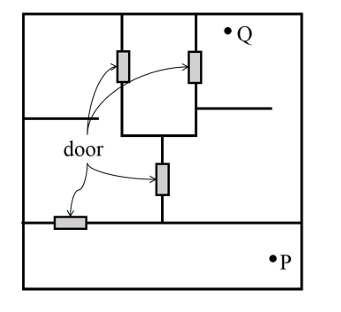
\includegraphics[width=0.5\columnwidth]{q5.png}
        \caption*{}
        \label{fig:q5}
    \end{figure}

    \hfill{\brak{\text{GATE GA 2022}}}
    \begin{enumerate}
        \begin{multicols}{4}
            \item $4$
            \item $3$
            \item $2$
            \item $1$
        \end{multicols}
    \end{enumerate}

    \item Rice, a versatile and inexpensive source of carbohydrate, is a critical component of diet worldwide. Climate change, causing extreme weather, poses a threat to sustained availability of rice. Scientists are working on developing Green Super Rice \brak{GSR}, which is resilient under extreme weather conditions yet gives higher yields sustainably. Which one of the following is the CORRECT logical inference based on the information given in the above passage?

    \hfill{\brak{\text{GATE GA 2022}}}
    \begin{enumerate}
        \item GSR is an alternative to regular rice, but it grows only in an extreme weather.
        \item GSR may be used in future in response to adverse effects of climate change.
        \item GSR grows in an extreme weather, but the quantity of produce is lesser than regular rice.
        \item Regular rice will continue to provide good yields even in extreme weather.
    \end{enumerate}

    \item A game consists of spinning an arrow around a stationary disk as shown below. When the arrow comes to rest, there are eight equally likely outcomes. It could come to rest in any one of the sectors numbered $1, 2, 3, 4, 5, 6, 7$ or $8$ as shown. Two such disks are used in a game where their arrows are independently spun. What is the probability that the sum of the numbers on the resulting sectors upon spinning the two disks is equal to $8$ after the arrows come to rest?
    \begin{figure}[h]
        \centering
        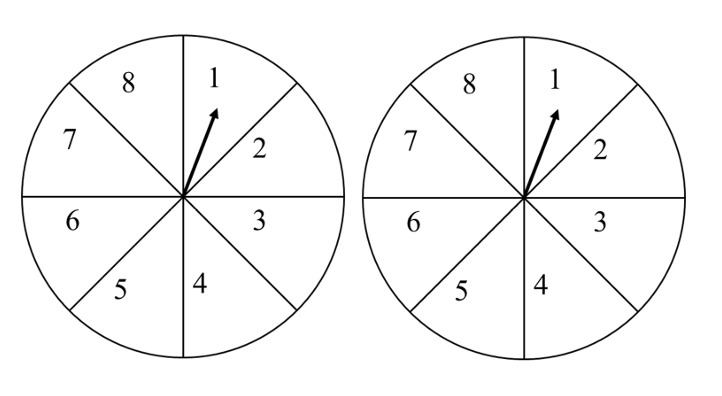
\includegraphics[width=0.4\columnwidth]{q7.png}
        \caption*{}
        \label{fig:q7}
    \end{figure}

    \hfill{\brak{\text{GATE GA 2022}}}
    \begin{enumerate}
        \begin{multicols}{4}
            \item $\frac{1}{16}$
            \item $\frac{5}{64}$
            \item $\frac{3}{32}$
            \item $\frac{7}{64}$
        \end{multicols}
    \end{enumerate}

    \item Consider the following inequalities.
    \begin{align*}
        3p - q < 4 \\
        3q - p < 12
    \end{align*}
    Which one of the following expressions below satisfies the above two inequalities?

    \hfill{\brak{\text{GATE GA 2022}}}
    \begin{enumerate}
        \begin{multicols}{2}
            \item $p+q < 8$
            \item $p+q = 8$
            \item $8 \le p+q < 16$
            \item $p+q \ge 16$
        \end{multicols}
    \end{enumerate}

    \item Given below are three statements and four conclusions drawn based on the statements.
    Statement 1: Some engineers are writers.
    Statement 2: No writer is an actor.
    Statement 3: All actors are engineers.
    Conclusion I: Some writers are engineers.
    Conclusion II: All engineers are actors.
    Conclusion III: No actor is a writer.
    Conclusion IV: Some actors are writers.
    Which one of the following options can be logically inferred?

    \hfill{\brak{\text{GATE GA 2022}}}
    \begin{enumerate}
        \item Only conclusion I is correct
        \item Only conclusion II and conclusion III are correct
        \item Only conclusion I and conclusion III are correct
        \item Either conclusion III or conclusion IV is correct
    \end{enumerate}

    \item Which one of the following sets of pieces can be assembled to form a square with a single round hole near the center? Pieces cannot overlap.
    
    \hfill{\brak{\text{GATE GA 2022}}}
    \begin{enumerate}
    \begin{figure}[H]
        \centering
        \item 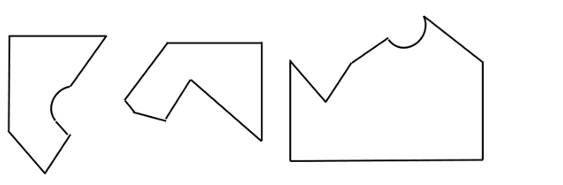
\includegraphics[width=0.4\columnwidth]{q10a.png}
        \item 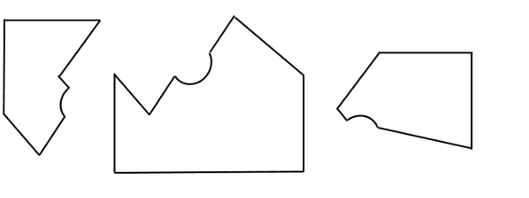
\includegraphics[width=0.4\columnwidth]{q10b.png}
        \item 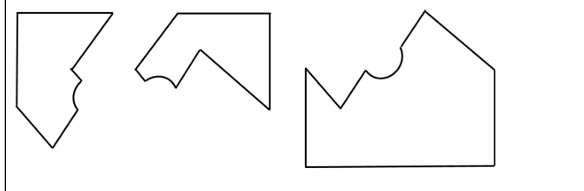
\includegraphics[width=0.4\columnwidth]{q10c.png}
        \item 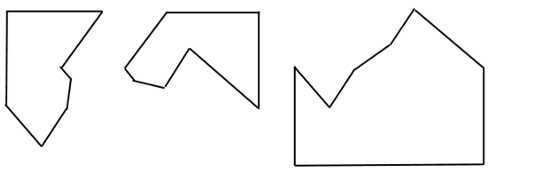
\includegraphics[width=0.4\columnwidth]{q10d.png}
        \caption*{}
        \label{fig:q10}
    \end{figure}
    \end{enumerate}

    \item If $a, b$ and $c$ are three vectors, the vector triple product $\brak{a\times b}\times c$ is given by

    \hfill{\brak{\text{GATE PI 2022}}}
    \begin{enumerate}
        \begin{multicols}{2}
            \item $\brak{a\cdot c}b-\brak{a\cdot b}c$
            \item $\brak{a\cdot b}c-\brak{a\cdot c}b$
            \item $\brak{a\cdot c}b-\brak{b\cdot c}a$
            \item $\brak{b\cdot c}a-\brak{a\cdot c}b$
        \end{multicols}
    \end{enumerate}

    \item The numerical integration of the function $y=2x+5$ is carried out between $x=1$ and $x=3$, by using ordinates at $x=1, 2$ and $3$. Which one of the following statements is TRUE?

    \hfill{\brak{\text{GATE PI 2022}}}
    \begin{enumerate}
        \item Simpson's $1/3$ rule will provide exact result but trapezoidal rule will not.
        \item Trapezoidal rule will provide exact result but Simpson's $1/3$ rule will not.
        \item Both Simpson's $1/3$ and trapezoidal rules will provide exact result.
        \item Neither Simpson's $1/3$ rule nor trapezoidal rule will provide exact result.
    \end{enumerate}

    \item Which one of the following metals has a face-centered cubic \brak{FCC} structure?

    \hfill{\brak{\text{GATE PI 2022}}}
    \begin{enumerate}
        \begin{multicols}{4}
            \item Alpha iron
            \item Chromium
            \item Magnesium
            \item Aluminum
        \end{multicols}
    \end{enumerate}

    \item If G denotes the shear modulus of an isotropic material, then the maximum possible value of Young's modulus of the material is

    \hfill{\brak{\text{GATE PI 2022}}}
    \begin{enumerate}
        \begin{multicols}{4}
            \item G
            \item 2 G
            \item 3 G
            \item 4 G
        \end{multicols}
    \end{enumerate}

    \item Match the casting methods with products.
    \begin{table}[h]
        \centering
        \caption*{}
        \label{tab:q15}
        \begin{tabular}{llcl}
            \hline
            \multicolumn{2}{l}{Casting method} & & Products \\
            \hline
            P & Continuous casting & 1 & Thin and intricate shaped components \\
            Q & Investment casting & 2 & Hollow axisymmetric parts \brak{such as pipes} \\
            R & Centrifugal casting & 3 & Slabs and strips \\
            \hline
        \end{tabular}
    \end{table}

    \hfill{\brak{\text{GATE PI 2022}}}
    \begin{enumerate}
        \begin{multicols}{4}
            \item P-3, Q-1, R-2
            \item P-2, Q-3, R-1
            \item P-3, Q-2, R-1
            \item P-2, Q-1, R-3
        \end{multicols}
    \end{enumerate}

    \item In injection blow molding of plastic beverage bottles, the blowing is accomplished by

    \hfill{\brak{\text{GATE PI 2022}}}
    \begin{enumerate}
        \begin{multicols}{4}
            \item hot water
            \item hot air
            \item hot oil
            \item alcohol
        \end{multicols}
    \end{enumerate}

    \item In an electro-discharge machining process, the discharge voltage is $V_b$. The energy dissipated per spark across the inter-electrode gap is proportional to

    \hfill{\brak{\text{GATE PI 2022}}}
    \begin{enumerate}
        \begin{multicols}{4}
            \item $0.5 V_b$
            \item $V_b$
            \item $2 V_b$
            \item $3 V_b$
        \end{multicols}
    \end{enumerate}

    \item Match the codes used in CNC part programming with their functions.
    \begin{table}[h]
        \centering
        \caption*{}
        \label{tab:q18}
        \begin{tabular}{llcl}
            \hline
            \multicolumn{2}{l}{Code} & & Function \\
            \hline
            P & G91 & 1 & End of program \\
            Q & M02 & 2 & Programming in incremental coordinates \\
            R & G32 & 3 & Spindle stop \\
            S & M05 & 4 & Thread cutting in turning \\
            \hline
        \end{tabular}
    \end{table}

    \hfill{\brak{\text{GATE PI 2022}}}
    \begin{enumerate}
        \begin{multicols}{2}
            \item P-2, Q-3, R-4, S-1
            \item P-2, Q-1, R-4, S-3
            \item P-4, Q-1, R-2, S-3
            \item P-4, Q-2, R-3, S-1
        \end{multicols}
    \end{enumerate}

    \item The control chart for a number of defects in a welded joint is

    \hfill{\brak{\text{GATE PI 2022}}}
    \begin{enumerate}
        \begin{multicols}{4}
            \item X chart
            \item R chart
            \item c chart
            \item p chart
        \end{multicols}
    \end{enumerate}

    \item Which one of the following statements is TRUE?

    \hfill{\brak{\text{GATE PI 2022}}}
    \begin{enumerate}
        \item Concurrent engineering is a non-integrated approach for designing a product.
        \item Concurrent engineering carries out all product development functions in a sequential manner.
        \item Concurrent engineering reduces the lead time for the product development.
        \item Concurrent engineering increases the lead time for the product development.
    \end{enumerate}

    \item Match the therblig symbols with their meanings.
    \begin{table}[H]
        \centering
        \caption*{}
        \label{tab:q21}
        \begin{tabular}{llcl}
            \hline
            \multicolumn{2}{l}{Therblig symbol} & & Meaning \\
            \hline
            P & 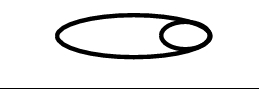
\includegraphics[width=0.02\columnwidth]{a21P.png} & 1 & Rest for overcoming fatigue \\
            Q & 
\includegraphics[width=0.02\columnwidth]{a21Q.png} & 2 & Avoidable delay \\
            R & 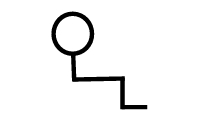
\includegraphics[width=0.02\columnwidth]{a21R.png} & 3 & Inspect \\
            S & 
\includegraphics[width=0.02\columnwidth]{a21S.png} & 4 & Search \\
            \hline
        \end{tabular}
    \end{table}

    \hfill{\brak{\text{GATE PI 2022}}}
    \begin{enumerate}
        \begin{multicols}{2}
            \item P-4, Q-3, R-1, S-2
            \item P-4, Q-3, R-2, S-1
            \item P-3, Q-4, R-1, S-2
            \item P-3, Q-4, R-2, S-1
        \end{multicols}
    \end{enumerate}

    \item Match the types of layout with the types of production.
    \begin{table}[h]
        \centering
        \caption*{}
        \label{tab:q22}
        \begin{tabular}{llcl}
            \hline
            \multicolumn{2}{l}{Type of layout} & & Type of production \\
            \hline
            P & Process layout & 1 & Job production \\
            Q & Product layout & 2 & Batch production \\
            R & Fixed position layout & 3 & Mass production \\
            \hline
        \end{tabular}
    \end{table}

    \hfill{\brak{\text{GATE PI 2022}}}
    \begin{enumerate}
        \begin{multicols}{2}
            \item P-2, Q-3, R-1
            \item P-3, Q-1, R-2
            \item P-2, Q-1, R-3
            \item P-3, Q-2, R-1
        \end{multicols}
    \end{enumerate}

    \item Matrix A as a product of two other matrices is given by
    \begin{align*}
        A = \myvec{3 & 1 \\ 4 & 2}
    \end{align*}
    The value of $\det\brak{A}$ is \underline{\hspace{2cm}}.

    \hfill{\brak{\text{GATE PI 2022}}}

    \item The order of the following differential equation is \underline{\hspace{2cm}}.
    \begin{align*}
        \brak{\frac{d^2y}{dx^2}}^3 + 5\frac{dy}{dx} + 4y = 5x
    \end{align*}

    \hfill{\brak{\text{GATE PI 2022}}}

    \item An operator manufactures $10$ identical spur gears in a lot. One spur gear is defective in the lot. Three spur gears are drawn at random without replacement. The probability of getting all three gears as non-defective is \underline{\hspace{2cm}}.

    \hfill{\brak{\text{GATE PI 2022}}}

    \item In a slider crank mechanism \brak{\text{schematic shown in the figure}}, the crank rotates at $60$ revolutions per minute. The radius of the crank is $30$ mm and the length of the connecting rod is $120$ mm. The average speed \brak{\text{in mm/s}} of the piston over one revolution of the crank is \underline{\hspace{2cm}}.
    \begin{figure}[H]
        \centering
        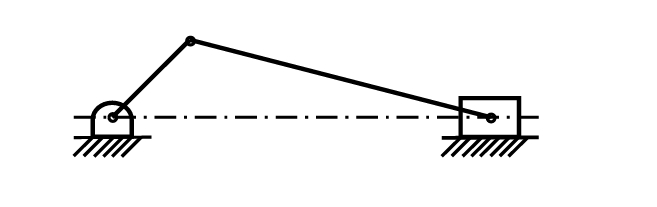
\includegraphics[width=0.6\columnwidth]{q26.png}
        \caption*{}
        \label{fig:q26}
    \end{figure}

    \hfill{\brak{\text{GATE PI 2022}}}

    \item Water \brak{\text{kinematic viscosity } \nu = 1 \times 10^{-6} m^2/s} is flowing through a circular horizontal pipe of diameter $8$ mm. If the flow is laminar and fully developed with a maximum axial velocity of $0.5$ m/s, the Reynolds number is \underline{\hspace{2cm}}.

    \hfill{\brak{\text{GATE PI 2022}}}

    \item Yielding starts in a material when the principal stresses are $100$ MPa, $100$ MPa and $-200$ MPa. As per the von Mises criterion, yield stress \brak{\text{in MPa}} of the material is \underline{\hspace{2cm}}.

    \hfill{\brak{\text{GATE PI 2022}}}

    \item A single-point cutting tool with zero rake angle is used for orthogonal machining. If the chip-compression ratio is $1.25$, then the shear angle \brak{\text{in degree}} during machining is \underline{\hspace{2cm}}.

    \hfill{\brak{\text{GATE PI 2022}}}

    \item It is required to cut a single-start thread of $2$ mm pitch in a lathe machine with a single-start lead screw of $4$ mm pitch. For one revolution of the workpiece, the number of revolution of the lead screw is \underline{\hspace{2cm}}.

    \hfill{\brak{\text{GATE PI 2022}}}
    \item The absolute deviations of $8$ points from the datum line of a surface are $10, 15, 12, 10, 13, 12, 20$ and $25$ $\mu$m. The root mean square value of the surface roughness \brak{\text{in } \mu\text{m}} is \underline{\hspace{2cm}}.

    \hfill{\brak{\text{GATE PI 2022}}}

    \item In a machine there are two motors, but only one motor is needed for the functioning of the machine. The reliabilities of the motors are $0.90$ and $0.70$. The overall reliability of the machine is \underline{\hspace{2cm}}.

    \hfill{\brak{\text{GATE PI 2022}}}

    \item If the interarrival time is exponential and $8$ customers per hour arrive in a bank, then the probability of no arrival of customer during a period of $15$ minutes is \underline{\hspace{2cm}}.

    \hfill{\brak{\text{GATE PI 2022}}}

    \item A company buys a machine worth Rs 65000, which has a salvage value of Rs 5000. The annual depreciation cost is Rs 10000 based on the straight line depreciation method. The useful life \brak{\text{in year}} of the machine is \underline{\hspace{2cm}}.

    \hfill{\brak{\text{GATE PI 2022}}}

    \item A project comprises of seven activities. The expected durations of activities and their variances are as follows:
    \begin{table}[h]
        \centering
        \caption*{}
        \label{tab:q35}
        \begin{tabular}{|c|c|c|}
            \hline
            Activity & Expected duration \brak{minute} & Variance \brak{minute} \\
            \hline
            A & $4$ & $1$ \\
            B & $5$ & $1$ \\
            C & $4$ & $1$ \\
            D & $1$ & $0$ \\
            E & $7$ & $4$ \\
            F & $6$ & $1$ \\
            G & $8$ & $4$ \\
            \hline
        \end{tabular}
    \end{table}
    The critical path consists of activities B, E and G. The standard deviation \brak{\text{in minute}} of the project duration is \underline{\hspace{2cm}}.

    \hfill{\brak{\text{GATE PI 2022}}}

    \item If a matrix is squared, then

    \hfill{\brak{\text{GATE PI 2022}}}
    \begin{enumerate}
        \item both eigenvalues and eigenvectors must change
        \item both eigenvalues and eigenvectors are retained
        \item eigenvalues get squared but eigenvectors are retained
        \item eigenvalues are retained but eigenvectors change
    \end{enumerate}

    \item Consider the following ordinary differential equation:
    \begin{align*}
        4\frac{d^{2}y}{dx^{2}}-4\frac{dy}{dx}+y=0.
    \end{align*}
    Given that $c_{1}$ and $c_{2}$ are constants, the general solution of the differential equation is

    \hfill{\brak{\text{GATE PI 2022}}}
    \begin{enumerate}
        \item $y=\brak{c_{1}+c_{2}x}e^{x}$
        \item $y=c_{1}e^{x/2}+c_{2}e^{x}$
        \item $y=c_{1}e^{x}+c_{2}e^{2x}$
        \item $y=\brak{c_{1}+c_{2}x}e^{x/2}$
    \end{enumerate}

    \item A market survey with a sample size of $1000$ was conducted for a parameter that follows normal distribution. The confidence interval was estimated as [$500, 700$] with a mean of $600$. It is now desired to reduce the confidence interval to [$550, 650$]. The sample size for achieving the desired interval at the same confidence level is

    \hfill{\brak{\text{GATE PI 2022}}}
    \begin{enumerate}
        \begin{multicols}{4}
            \item $1000$
            \item $4000$
            \item $9000$
            \item $16000$
        \end{multicols}
    \end{enumerate}

    \item A eutectoid steel with $100\%$ austenite is cooled from a temperature of $750\degree$C to a room temperature of $35\degree$C. Match the cooling methods with transformed structures.
    \begin{table}[h]
        \centering
        \caption*{}
        \label{tab:q39}
        \begin{tabular}{llll}
            \hline
            \multicolumn{2}{l}{Cooling method} & \multicolumn{2}{l}{Transformed structure} \\
            \hline
            P & Water quenching & 1 & Coarse pearlite \\
            Q & Oil quenching & 2 & Fine pearlite \\
            R & Air cooling & 3 & Martensite \\
            S & Furnace cooling & 4 & Very fine pearlite \\
            \hline
        \end{tabular}
    \end{table}

    \hfill{\brak{\text{GATE PI 2022}}}
    \begin{enumerate}
        \begin{multicols}{2}
            \item P-1, Q-2, R-3, S-4
            \item P-2, Q-3, R-4, S-1
            \item P-3, Q-4, R-2, S-1
            \item P-3, Q-4, R-1, S-2
        \end{multicols}
    \end{enumerate}

    \item In the three-member truss shown in the figure, $AC=BC$. An external force of $10$ kN is applied at B, parallel to AC. The force in the member BC is
    \begin{figure}[h]
        \centering
        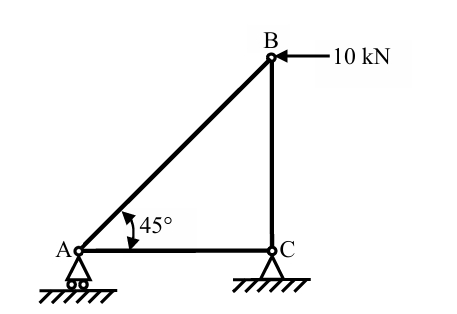
\includegraphics[width=0.4\columnwidth]{q40.png}
        \caption*{}
        \label{fig:q40}
    \end{figure}

    \hfill{\brak{\text{GATE PI 2022}}}
    \begin{enumerate}
        \item zero
        \item $10$ kN \brak{\text{tensile}}
        \item $10$ kN \brak{\text{compressive}}
        \item $7.07$ kN \brak{\text{tensile}}
    \end{enumerate}

    \item Match the processing steps related to production of powder metallurgy parts with their descriptions.
    \begin{table}[h]
        \centering
        \caption*{}
        \label{tab:q41}
        \begin{tabular}{llcl}
            \hline
            \multicolumn{2}{l}{Processing step} & & Description \\
            \hline
            P & Atomization & 1 & Blended powders are pressed into shapes using dies and pressure \\
            Q & Sintering & 2 & A process for producing metal powder \\
            R & Compaction & 3 & Metal powders are heated below their melting points to allow bonding \\
            S & Infiltration & 4 & A slug of low melting point metal is placed in contact with the sintered part and heated \\
              &             & 5 & Metal powders are heated significantly above their melting points for bonding \\
            \hline
        \end{tabular}
    \end{table}

    \hfill{\brak{\text{GATE PI 2022}}}
    \begin{enumerate}
        \begin{multicols}{2}
            \item P-1, Q-5, R-2, S-3
            \item P-3, Q-2, R-1, S-5
            \item P-2, Q-3, R-1, S-4
            \item P-2, Q-5, R-1, S-4
        \end{multicols}
    \end{enumerate}

    \item In an assembly comprising shaft and hole, the nominal sizes with tolerances are specified as
    \begin{align*}
        \text{Hole: } 25.000^{+0.002}_{-0.001} \text{ mm,} \\
        \text{Shaft: } 25.000^{+0.001}_{-0.003} \text{ mm.}
    \end{align*}
    The type of fit is

    \hfill{\brak{\text{GATE PI 2022}}}
    \begin{enumerate}
        \item Clearance fit
        \item Interference fit
        \item Transition fit
        \item Running fit
    \end{enumerate}

    \item In a manufacturing system, four different types of products \brak{P, Q, R and S} are produced. The batch size of each product is $2 \times 10^{7}$. The numbers of defective units are $60, 71, 80$ and $55$, for P, Q, R and S, respectively. Which one of the following statements is TRUE?

    \hfill{\brak{\text{GATE PI 2022}}}
    \begin{enumerate}
        \item All products conform to six sigma standard.
        \item Only product S conforms to six sigma standard.
        \item Except R, all other products conform to six sigma standard.
        \item Products P and S conform to six sigma standard.
    \end{enumerate}

    \item Match the processes of product development with their characteristics.
    \begin{table}[h]
        \centering
        \caption*{}
        \label{tab:q44}
        \begin{tabular}{llcl}
            \hline
            \multicolumn{2}{l}{Process} & & Characteristic \\
            \hline
            P & Product synthesis & 1 & Process of conversion of conceptual design into engineering science based model \\
            Q & Product simplification & 2 & Process related to design conceptualization \\
            R & Product analysis & 3 & Process of maintaining uniformity and consistency \\
            S & Product standardization & 4 & Process of reducing the number of parts without losing the functionalities \\
            \hline
        \end{tabular}
    \end{table}

    \hfill{\brak{\text{GATE PI 2022}}}
    \begin{enumerate}
        \begin{multicols}{2}
            \item P-2, Q-4, R-1, S-3
            \item P-2, Q-3, R-1, S-4
            \item P-4, Q-3, R-1, S-2
            \item P-4, Q-3, R-2, S-1
        \end{multicols}
    \end{enumerate}
    \item The value of
    \begin{align*}
        \lim_{x\rightarrow1}\frac{x^{3}-3x+2}{x^{3}-x^{2}-x+1}
    \end{align*}
    is \underline{\hspace{2cm}}.

    \hfill{\brak{\text{GATE PI 2022}}}

    \item A thick-cylinder has inner diameter of $20$ mm and outer diameter of $40$ mm. It is subjected to an internal pressure of $100$ MPa. Follow the convention of taking tensile stress as positive and compressive stress as negative. The sum of radial and hoop stresses \brak{\text{in MPa}} at a radius of $15$ mm is \underline{\hspace{2cm}}.

    \hfill{\brak{\text{GATE PI 2022}}}

    \item A shaft is used to transmit a power of $10$ kW. The shear yield stress of the material is $150$ MPa and factor of safety is $2$. The shaft rotates at $1440$ revolutions per minute. The diameter of the shaft \brak{\text{in mm}} based on static strength is \underline{\hspace{2cm}}.

    \hfill{\brak{\text{GATE PI 2022}}}

    \item Air at an initial temperature and pressure of $15\degree$C and $1$ bar, respectively is heated in an irreversible process. The final temperature and pressure are $303\degree$C and $2$ bar, respectively. Take gas constant for air as $R=287$ J/kg-K, the ratio of the specific heats as $\gamma=1.4$ and treat air as a calorically perfect gas. The change of entropy \brak{\text{in J/kg-K}} in the process is \underline{\hspace{2cm}}.

    \hfill{\brak{\text{GATE PI 2022}}}

    \item During a hot-working process, the homologous temperature is $0.8$. The melting point of the work metal is $800\degree$C. The temperature \brak{\text{in }\degree\text{C}} during hot-working is \underline{\hspace{2cm}}.

    \hfill{\brak{\text{GATE PI 2022}}}

    \item A workpiece of $30$ mm diameter and $40$ mm height is compressed between two platens in an open die forging process. Assume a perfectly plastic material with a flow stress of $300$ MPa. The ideal forging load \brak{\text{in kN}} at $30\%$ reduction \brak{\text{in height}} is \underline{\hspace{2cm}}.

    \hfill{\brak{\text{GATE PI 2022}}}

    \item In a gas tungsten arc welding process under steady state condition, the input voltage and current are measured as $18$ V and $160$ A, respectively. Heat loss during creation of arc is $40\%$ of the input power. Heat loss through convection and radiation from the workpiece is $800$ W. The effective power \brak{\text{in W}} utilized to melt the workpiece is \underline{\hspace{2cm}}.

    \hfill{\brak{\text{GATE PI 2022}}}

    \item During straight turning of a $20$ mm diameter steel bar at a spindle speed of $400$ revolutions per minute \brak{RPM} with an HSS tool, a tool life of $10$ minute was observed. When the same bar was turned at $200$ RPM, the tool life increased to $40$ minute. The tool life \brak{\text{in minute}} while machining the bar at $300$ RPM is \underline{\hspace{2cm}}.

    \hfill{\brak{\text{GATE PI 2022}}}

    \item A cylindrical workpiece is turned using two different tools. Tool 1 has zero nose radius; side and end cutting edge angles are $20\degree$ and $10\degree$, respectively. Tool 2 has $0.5$ mm nose radius. Both the tools machine at a feed of $0.2$ mm/rev. The ratio of ideal maximum height of unevenness on the surface produced by Tool 1 to that produced by Tool 2 is \underline{\hspace{2cm}}.

    \hfill{\brak{\text{GATE PI 2022}}}

    \item For an electrochemical machining process
    \begin{align*}
        \frac{dy}{dt}=\frac{\lambda}{y}-f,
    \end{align*}
    where y is the inter-electrode gap in mm at time t in minute, and f is the feed of the tool in mm/minute. The value of $\lambda$ is $6\times10^{-3} \text{cm}^{2}/\text{minute}$. For maintaining a constant inter-electrode gap of $0.1$ mm, the feed \brak{\text{in mm/minute}} should be \underline{\hspace{2cm}}.

    \hfill{\brak{\text{GATE PI 2022}}}

    \item The worktable of an open loop positioning system is driven by a lead screw with a pitch of $4$ mm. The lead screw is connected to the shaft of a stepper motor. A gear of $80$ teeth mounted on the stepper motor shaft meshes with a gear of $20$ teeth mounted on the lead screw. The step angle of the stepper motor is $9\degree$. The number of pulses required to move the table by $200$ mm is \underline{\hspace{2cm}}.

    \hfill{\brak{\text{GATE PI 2022}}}

    \item The diameter of a cylindrical cavity is measured by using two spherical steel balls of diameters $3$ cm and $4$ cm. The balls are placed inside the cavity such that the bigger ball is above the smaller one as shown in the figure. If the depth of cavity is $6$ cm, then the diameter \brak{\text{in cm}} of cavity is \underline{\hspace{2cm}}.
    \begin{figure}[h]
        \centering
        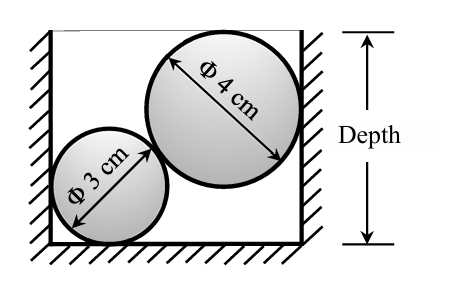
\includegraphics[width=0.4\columnwidth]{q56.png}
        \caption*{}
        \label{fig:q56}
    \end{figure}

    \hfill{\brak{\text{GATE PI 2022}}}

    \item In a mobile screen manufacturing process on a mass scale basis, $5$ samples of size $80$ are inspected. Consider a p-chart with $\pm3\sigma$ limits \brak{\sigma is the standard deviation}. The numbers of defective items are given in the table.
    \begin{table}[H]
        \centering
        \caption*{}
        \label{tab:q57}
        \begin{tabular}{|c|c|}
            \hline
            Sample No. & Number of defective items \\
            \hline
            1 & 4 \\
            2 & 10 \\
            3 & 5 \\
            4 & 6 \\
            5 & 5 \\
            \hline
        \end{tabular}
    \end{table}
    The upper control limit of the defective item \brak{\text{in fraction defective}} is \underline{\hspace{2cm}}.

    \hfill{\brak{\text{GATE PI 2022}}}

    \item In a factory, $100$ bulbs are in use. The table lists the cumulative probability of the failure of a bulb for various durations.
    \begin{table}[h]
        \centering
        \caption*{}
        \label{tab:q58}
        \begin{tabular}{|c|c|}
            \hline
            Duration \brak{month} & Cumulative probability \\
            \hline
            1 & 0.10 \\
            2 & 0.25 \\
            3 & 0.47 \\
            4 & 0.68 \\
            5 & 1.00 \\
            \hline
        \end{tabular}
    \end{table}
    The factory follows the individual replacement policy. If the cost of replacing a bulb is Rs 300, then the expected cost \brak{\text{in Rs}} of replacement per month is \underline{\hspace{2cm}}.

    \hfill{\brak{\text{GATE PI 2022}}}

    \item A company procures $384$ parts annually. The annual holding cost per part is Rs 30. If the ordering cost is Rs 1000, then the economic order quantity is \underline{\hspace{2cm}}.

    \hfill{\brak{\text{GATE PI 2022}}}

    \item A time study engineer recorded the cycle time \brak{\text{in minute}} for machining of a component. The recorded time study data is provided in the table. The performance rating of the worker is $110\%$. The standard time for machining \brak{\text{in minute}} the component by assuming $10\%$ allowance is \underline{\hspace{2cm}}.
    \begin{table}[h]
        \centering
        \caption*{}
        \label{tab:q60}
        \begin{tabular}{|c|c|}
            \hline
            Cycle time \brak{minute} & Frequency \\
            \hline
            42 & 1 \\
            43 & 2 \\
            44 & 3 \\
            45 & 2 \\
            46 & 1 \\
            \hline
        \end{tabular}
    \end{table}

    \hfill{\brak{\text{GATE PI 2022}}}

    \item A machine component is to be processed at $5$ workstations sequentially. The table provides the cycle time \brak{\text{in second}} of each workstation. In mass production, the number of components produced per hour \brak{\text{in steady state}} is \underline{\hspace{2cm}}.
    \begin{table}[h]
        \centering
        \caption*{}
        \label{tab:q61}
        \begin{tabular}{|c|c|}
            \hline
            Workstation & Cycle time of each workstation \brak{second} \\
            \hline
            WS-1 & 85 \\
            WS-2 & 55 \\
            WS-3 & 90 \\
            WS-4 & 65 \\
            WS-5 & 70 \\
            \hline
        \end{tabular}
    \end{table}

    \hfill{\brak{\text{GATE PI 2022}}}

    \item A vaccine has to be distributed from two warehouses to three hospitals. The supplies at warehouses $W_{1}$ and $W_{2}$ are $200$ and $150$, respectively. The demands at hospitals $H_{1}$, $H_{2}$, and $H_{3}$ are $100$, $150$ and $125$, respectively. The transportation cost \brak{\text{in Rs}} per vaccine is as follows:
    \begin{table}[H]
        \centering
        \caption*{}
        \label{tab:q62}
        \begin{tabular}{cccc}
            & $H_{1}$ & $H_{2}$ & $H_{3}$ \\
            $W_{1}$ & 5 & 7 & 3 \\
            $W_{2}$ & 4 & 6 & 7 \\
        \end{tabular}
    \end{table}
    The initial basic feasible solution using the Northwest-corner method provides the total transportation cost \brak{\text{in Rs}} as \underline{\hspace{2cm}}.

    \hfill{\brak{\text{GATE PI 2022}}}

    \item Consider the linear programming problem:
    \begin{align*}
        \text{Maximize } z=20x_{1}+6x_{2}+Px_{3}, \\
        \text{subject to} \\
        \text{\brak{C1} } 8x_{1}+2x_{2}+3x_{3}\le250, \\
        \text{\brak{C2} } 4x_{1}+3x_{2}\le150, \\
        \text{\brak{C3} } 2x_{1}+x_{3}\le50, \\
        x_{1}, x_{2}, x_{3}\ge0
    \end{align*}
    The optimal solution is given as $x_{1}^{}=0$, $x_{2}^{}=50$ and ${x_{3}}^{}=50$. The dual variables of constraints $C_{1}$, $C_{2}$ and $C_{3}$ are $y_{1}$, $y_{2}$ and $y_{3}$, respectively. The optimal values of dual variables are $y_{1}^{}=0$, $y_{2}^{}=2$ and $y_{3}^{}=8$. The value of parameter P in the objective function is \underline{\hspace{2cm}}.

    \hfill{\brak{\text{GATE PI 2022}}}

    \item A company is planning to produce $24$ electric cars per day. The setup cost of the plant is estimated as Rs 19476 million and the variable cost is Rs 0.6 million per car. The car will be sold at a price of Rs 1.5 million. The number of days required for achieving the breakeven is \underline{\hspace{2cm}}.

    \hfill{\brak{\text{GATE PI 2022}}}

    \item A company forecasts the weekly demand of oxygen cylinders using exponential smoothing method with smoothing constant $\alpha=0.2$. The actual demands in Week 1, Week 2, Week 3 and Week 4 were $375$, $412$, $592$ and $439$ units, respectively. The forecasted demand for Week 3 was $500$ units. The forecast \brak{\text{in unit}} for the Week 5 is \underline{\hspace{2cm}}.

    \hfill{\brak{\text{GATE PI 2022}}}
    
\end{enumerate}

\end{document}